% 
% Annual Cognitive Science Conference
% Sample LaTeX Paper -- Proceedings Format
% 

% Original : Ashwin Ram (ashwin@cc.gatech.edu)       04/01/1994
% Modified : Johanna Moore (jmoore@cs.pitt.edu)      03/17/1995
% Modified : David Noelle (noelle@ucsd.edu)          03/15/1996
% Modified : Pat Langley (langley@cs.stanford.edu)   01/26/1997
% Latex2e corrections by Ramin Charles Nakisa        01/28/1997 
% Modified : Tina Eliassi-Rad (eliassi@cs.wisc.edu)  01/31/1998
% Modified : Trisha Yannuzzi (trisha@ircs.upenn.edu) 12/28/1999 (in process)
% Modified : Mary Ellen Foster (M.E.Foster@ed.ac.uk) 12/11/2000
% Modified : Ken Forbus                              01/23/2004
% Modified : Eli M. Silk (esilk@pitt.edu)            05/24/2005
% Modified: Niels Taatgen (taatgen@cmu.edu) 10/24/2006

%% Change ``a4paper'' in the following line to ``letterpaper'' if you are
%% producing a letter-format document.

\documentclass[10pt,letterpaper]{article}
\usepackage{graphicx}
\usepackage{cogsci}
\usepackage{pslatex}
\usepackage{apacite}


\title{The Pragmatics of Metaphor Understanding: A Computational Approach}
 
\author{{\large \bf Justine T. Kao (justinek@stanford.edu)} \\
  Department of Psychology\\
  Stanford, CA, USA
   \AND {\large \bf Leon Bergen (bergen@mit.edu)} \\
  Department of Brain and Cognitive Sciences\\
 MIT, USA
  \AND {\large \bf Noah D. Goodman (ngoodman@stanford.edu)} \\
  Department of Psychology\\
  Stanford, CA, USA}


\begin{document}

\maketitle


\begin{abstract}
Abstract goes here.
%Metaphor understanding has been widely studied in psychology, linguistics, philosophy, and computer science. One account of metaphor understanding is pragmatics. Some metaphor interpretations arise from pragmatics. Here we present a computational model of pragmatics that accounts for 

\textbf{Keywords:} 
language understanding; metaphor; pragmatics; computational models
\end{abstract}


\section{Introduction}
Nonliteral language is, quite literally, everywhere. Human communication is laden with metaphor, irony, and hyperbole, often creating poetic or humorous effects that add rich and important dimensions to language. Of the various types of nonliteral language, metaphor has inspired a particularly abundant amount of research in cognitive science, ranging from how metaphors structure and shape our thoughts (cite), whether metaphor processing recruits the same strategies as standard language processing (cite), and what factors determine the meaning and aptness of a novel metaphor (cite). The overwhelming amount of interest in metaphor research is due in part to the ubiquity of metaphor in everyday language as well as the increasingly popular belief that metaphor may be critical for helping us understand how the mind creates meaning. 

One area of research focuses on the pragmatic principals that listeners utilize to infer meaning from metaphorical utterances in context. Rather than viewing metaphor as a separate mode of communication that requires specialized language processing strategies, this approach argues that basic principles of communication drive the meaning that a listener infers from a metaphorical sentence. Relevance theory, in particular, explains metaphor understanding and communication in general with the assumption that human cognition is shaped by evolution to maximize relevance. Based on this theory, a listener interprets an utterance with the assumption that it is the most relevant utterance that the communicator chose to produce. Relevance theorists argue that this principle explains how listeners infer the intended meaning from a novel metaphor. To interpret the sentence ``My lawyer is a shark," for example, the listener assumes that the speaker only aims to communicate features of ``a shark" that are relevant to the topic ``my lawyer." Under such a view, metaphors are a subset of the more general phenomenon of ``loose talk", where speakers can use a term loosely with the expectation that the principle of relevance will help listeners infer the correct meaning. 

While many linguists and psychologists have argued for the importance of studying metaphor using a pragmatics framework, the work has been largely qualitative. As a result, it has been difficult to formally show that effects in metaphor understanding may arise from adhering to basic principles of pragmatics. On the other hand, a recent body of work computationally models language understanding as probabilistic social inference, where speaker and listener recursively reason about each other to communicate effectively. By formalizing principals of communication, these Rational Speech Act models are able to quantitatively explain a range of phenomena in human pragmatic reasoning, such as scalar implicature and the effect of considering alternative utterances. However, a limitation of these models is that they are unable to predict interpretations of an utterance that are false under its literal meaning. In more recent work, we extended this model to consider situations where the listener is uncertain about the speaker's communicative goal and performs joint inference on both the goal and the intended meaning. Under such a framework, the space of meanings has multiple dimensions, and each dimension may satisfy a different communicative goal. A speaker's goal may be to maximize the informativeness of her utterance along one dimension of meaning but not another given her communicative goal. This makes it possible for a literally false utterance to be optimal as long as it is informative along the target dimension. Critically, this framework aligns with the relevance-theoretic view that certain aspects of a metaphor's meaning are more relevant than others and thus should be judged as more likely by the listener.

Although metaphor understanding is a complex phenomenon that calls for a variety of approaches, here we argue that the interpretation of at least some types of metaphor are shaped at least in part by basic principals of pragmatics. In particular, we focus on metaphors of the classic form ``$X$ is a $Y$." Building upon Rational Speech Act models, we present a computational model showing that rich metaphorical meaning can arise from basic pragmatic principals. We conduct behavioral experiments to demonstrate three effects in metaphor understanding: (1) A listener's interpretation of a metaphor relies on prior knowledge of both the target (lawyer) and the source (shark). (2) A listener's interpretation of a metaphor is driven by context and the question under discussion (e.g., ``My lawyer is a shark" is interpreted differently if preceded by the question ``Is your lawyer fierce?" or ``Is your lawyer a good swimmer?") (3) Metaphors often communicate information more efficiently than literal statements and hence can be optimal and rational speech acts. [Plus whatever we end up focusing on in the error analysis]

\section{Computational Model}
At the core of basic Rational Speech Act models, a listener and a speaker recursively reason about each other to arrive at pragmatically enriched meanings. Given an intended meaning $m$, a speaker $S_n$ reasons about a listener $L_{n-1}$ and chooses utterance $u$ based on its informativeness:
$$
S_n (u|m)\propto L_{n-1} (m|u) e^{c(u)}
$$
The listener $L_n$ then reasons about $S_n$ and uses Bayes� Rule to infer the meaning $m$ given the utterance $u$:
$$
L_n (m|u)\propto P(m)S_n (u|m)
$$
We extend this model by formalizing a notion of relevance using communicative goals. Different utterances may be optimally informative given different goals during communication, which is consistent with the idea that a speaker aims not only to be informative, but also relevant. Metaphors of the form ``$X$ is a $Y$" are argued by some metaphor researchers to be class-inclusion assertions. Although we do not make theoretical commitments with regards to this argument, we model the space of meanings as involving categories and their features. For example, ``shark" is a category, and ``fierce" and "dangerous" are potential features. As a result, the interpreted meaning of the sentence ``$X$ is a $Y$" consists of the category $c$ to which $X$ belongs and the values of the features that $X$ has. For simplicity, in this model we restrict the number of possible categories to two: $c_a$ and $c_p$. We also restrict the number of possible communicative goals $g$ and features under consideration $f$ to three. If the speaker has a goal $g_i$, she wishes to maximize informativeness about $f_i$. We will use $f$ as a shorthand for the values of the featurs $f_1, f2, f3$.
% I need help with this....(Formally, the goal $g_i$ is a function $g_i: M \rightarrow\{0, 1\}$, such that $g_i(f) = 1$ if and only if)
Under this formulation, 
$$
S_n (u | g) \propto e^{U_n (u | g)}
$$
Optimizing the probability of the speaker's goal being satisfied can be accomplished by minimizing the goal�s information-theoretic surprisal of her goal given an utterance. Given an utterance u, the listener $L_n$ will guess that the meaning is $c, f$ with probability $L_n (c, f|u)$. The probability of the speaker�s goal being satisfied is therefore the following:
$$
\sum_{c, f}{L_n (c, f|u) g(f)}
$$
The utility function $U_n$ is composed of both the negative surprisal of the goal and the negative of the utterance cost $C(u)$.  $U_n$ is therefore defined by:
$$
U_n (u|g)= \log (?{\sum_{c, f}{L_n (c,f|u) g(c,f))-C(u)}})
$$
Combined with equation 2 and using a uniform utterance cost, this leads to:
$$
S_n (u | g) \propto \sum_{c,f}{L_n (c,f|u) g(c,f)}
$$

The listener $L_n$ performs Bayesian inference to guess the intended meaning given the prior P and his internal model of the speaker. To determine the speaker's intended meaning, the listener will marginalize over the possible goals under consideration.
$$
L_n (c,f | u) \propto \sum_{g}{P_C (c) P_F (f | c) P_G (g|c, f) S_{n-1} (u|g)}
$$
Note that the listener needs to consider the following prior probabilities: 
\begin{itemize}
\item[(1)] $P_C(c)$, the prior probability that $X$ belongings category $c$. We assume that $X$ belongs to $c_p$ with very high probability. 
\item[(2)] $P_F(f | c)$, the prior probability that a member of category $c$ has feature values $f$. We obtain this empirically in Experiment 1.
\item[(3)] $P_G(g | c, f)$, the prior probability that given that a speaker knows the meaning $c, f$, she wishes to communicate goal $g$. We assume that this prior can change given the question under discussion, i.e. the context that a question sets up.
\end{itemize}

\section{Behavioral Experiments}
In order to obtain human metaphorical interpretations that we can compare against our model, we focused on a set of metaphors in which a male human is the target and a non-human animal is the source. We selected $32$ common non-human animal categories. Using this list, we conducted Experiment 1A to elicit a set of three salient features for each animal category. We conducted Experiment 1B to elicit the feature priors $P_F(f | c)$ described in the model section (see Table 1). Finally, we conducted Experiment 2 to measure people's interpretations of the set of metaphors. 

\subsection{Experiment 1A: Feature Elicitation}
\subsubsection{Materials and Methods}
$100$ native English speakers with IP addresses in the United States were recruited on Amazon's Mechanical Turk for the first part of the feature prior elicitation experiment. Each subject read $32$ animal terms presented in random order. For each animal term, subjects were asked to type the first adjective that came to mind in a text box. 
\subsubsection{Results}
For each animal category, we constructed a list of adjectives that the subjects gave and ordered them by popularity. We removed all color adjectives, such as ``brown" and ``black." To avoid constructing a set of features that have roughly equivalent meanings such as ``big", ``huge", and ``large", we used Wordnet to identify synonyms and only kept the most popular one among a set of synonymous adjectives. We then took the top three most popular adjectives for each animal category and used them as the set of features. Note that $f_1$ is the most popular adjective, $f_2$ the second, and $f_3$ the third. Table 1 shows the animal categories and their respective features.
\subsection{Experiment 1B: Feature Prior Elicitation}
\subsubsection{Materials and Methods}
We used Wordnet to construct antonyms for each of the adjective features produced in Experiment 1A. When multiple antonyms existed or when no antonym could be found on Wordnet, the first author used her judgment to choose the appropriate antonym. Table 1 shows the resulting list of antonyms. For each animal category, eight possible feature combinations were constructed from the three features and their antonyms. For example, the possible feature combinations for a member of the category \emph{ant} are \{small, strong, busy\}, \{small, strong, idle\}, \{small, weak, busy\}, and so on.

$60$ native English speakers with IP addresses in the United States were recruited on Amazon's Mechanical Turk for the second part of the feature prior elicitation experiment. Each subject completed $16$ randomly selected trials in random order. Each trial consisted of the eight feature combinations for a particular animal category (e.g. \emph{ant}). Using slider bars ranging from ``Impossible" to ``Absolutely certain," subjects were asked to rate how likely it is for a member of the animal category to have each of the eight feature combinations. Subjects also rated the probabilities of the feature combinations for a male person.

\subsubsection{Results} 
We make the simplifying assumption that the eight feature combinations presented in each trial represent all possible features combinations of a member of a particular category. As a result, we normalized each subject's ratings for the eight feature combinations of a member of a category to sum up to 1. Averaging across subjects' normalized ratings, we obtained the feature priors $P_F(f | c)$ for $c = c_a$ (animal) and $c = c_p$ (person). For ease of interpretation, in Table 1 we present the marginal probabilities for each of the three features instead of the joint probabilities. Figure~\ref{prior} shows the average marginal probabilities of features given an animal category versus a person category. We see that by design, features are rated as significantly more likely to be present given the animal category than the person category.

\begin{figure}[h]
\begin{center}
\scalebox{0.6}{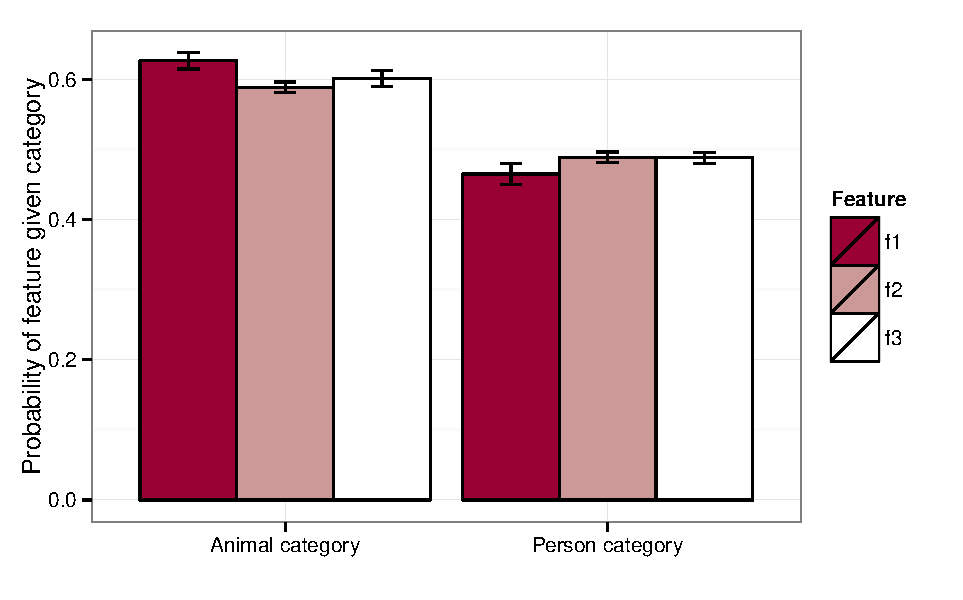
\includegraphics{Plots/prior.pdf}}
\end{center}
\caption{This is a figure.} 
\label{prior}
\end{figure}

\subsection{Experiment 2: Metaphor Understanding}
\subsubsection{Materials and Methods}
We created $32$ scenarios using the animal categories. In each scenario, a person (e.g. Bob) is having a conversation with his friend about a person that he recently met. Since we are interested how relevance to the question under discussion (QUD) affects interpretation as well as the effectiveness of metaphorical versus literal statements, we created four conditions for each scenario by crossing Vague/Specific QUD and Literal/Metaphorical statements. In Vague QUD conditions, Bob's friend asks a vague question about the person Bob recently met: ``What is he like?" In Specific QUD conditions, Bob's friend asks a specific question about the person: ``Is he $f_1$?" Where $f_1$ is the most popular adjective for a given animal category $c_a$ in Experiment 1A. In Literal conditions, Bob replies with a literal statement, either by saying ``He is $f_1$" to the question ``What is he like?" or ``Yes" to the question ``Is he $f_1$?". In Metaphorical conditions, Bob replies with a metaphorical statement, e.g. ``He is a $c_a$" where $c_a$ is an animal category. See Table 2 for examples.
 
$49$ native English speakers with IP addresses in the United States were recruited on Amazon's Mechanical Turk. Each subject completed $32$ trials in random order. The $32$ trials were randomly and evenly assigned to one of the four conditions, i.e. each subject read $8$ scenarios for each condition. For each trial, subjects used sliders to indicate the probabilities that the person described has features $f_1$, $f_2$, and $f_3$.

\subsubsection{Results}
For each condition of each scenario, we obtained the average probability ratings for each of the features under consideration. Figure \ref{human_bar} shows the average ratings for each feature across animal categories given a vague or specific QUD and a literal or metaphorical utterance. We see that when the speaker gives a literal statement directly affirming the presence of $f_1$, subjects rate $f_1$ as significantly more likely than when the speaker gives a metaphorical statement. However, subjects rate $f_2$ and $f_3$ as significantly more likely when the speaker produces a metaphorical utterance. We also see an effect of the QUD for metaphorical utterances. Given a specific question about $f_1$, subjects interpret the speaker's metaphorical utterance as being relevant to the question and rates the probability of $f_1$ as significantly higher than when the QUD is vague. On the other hand, the probabilities of $f_2$ and $f_3$ are not significantly different given a vague or specific QUD about $f_1$.
\begin{figure}[h]
\begin{center}
\scalebox{0.6}{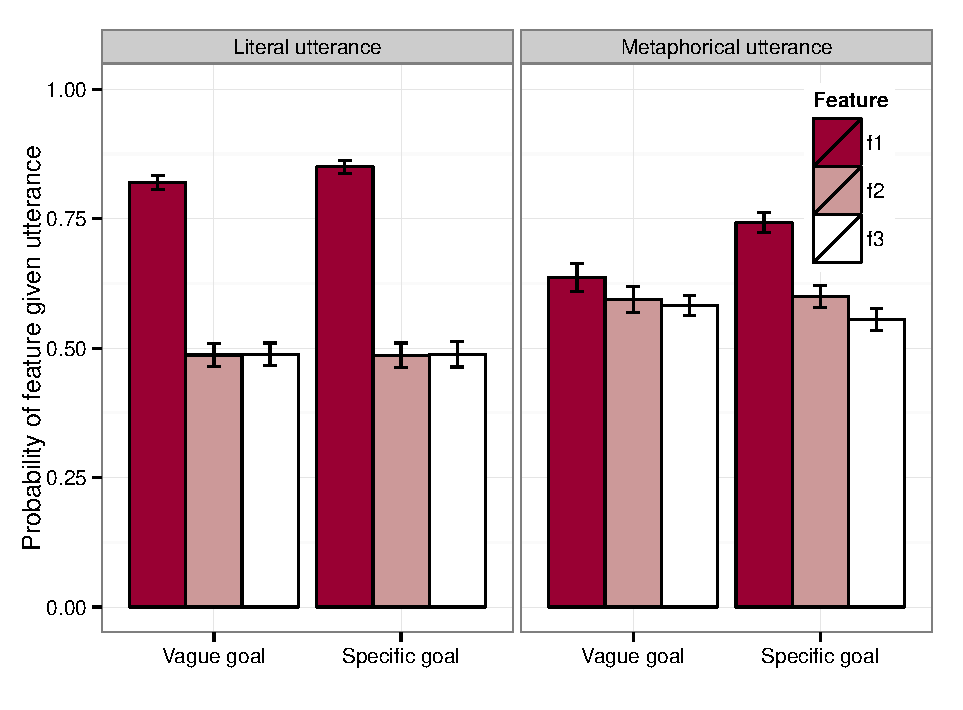
\includegraphics{Plots/human_bar.pdf}}
\end{center}
\caption{This is a figure.} 
\label{human_bar}
\end{figure}

\section{Model Comparison}
We used the feature priors obtained in Experiment 1B to compute model interpretations of the $32$ metaphors.
For the category prior $P_C(c)$, we assumed that given the common ground set up by the conversation, it is extremely unlikely for the person described to actually belong to the animal category $(P_C(c_a) = 0.0001)$ and extremely likely for him to belong to the person category $(P_C(c_p) = 0.9999)$. We model the effect of relevance to the question under discussion by assuming that the goal prior $P_G(g | c, f)$ varies given vague or specific QUDs. When the QUD is vague, we set the distribution as uniform over goals that are consistent with $c, f$. When the QUD specifically addresses $f_1$, we set the distribution as having a much higher probability for $g_1$ and equal probability for $g_2$ and $g_3$.

Using these prior settings and the model we described, we obtained feature probabilities for each of the $32$ metaphors. Figure~\ref{model_bar} shows the average marginal feature probabilities for the $32$ metaphors given a vague or specific QUD. We see that the model captures the QUD effect, where $f_1$ receives a significantly higher probability when the speaker is a priori more likely to be informative about $f_1$.
% should show results for "literal" statement where it's just the prior.
\begin{figure}[ht]
\begin{center}
\scalebox{0.6}{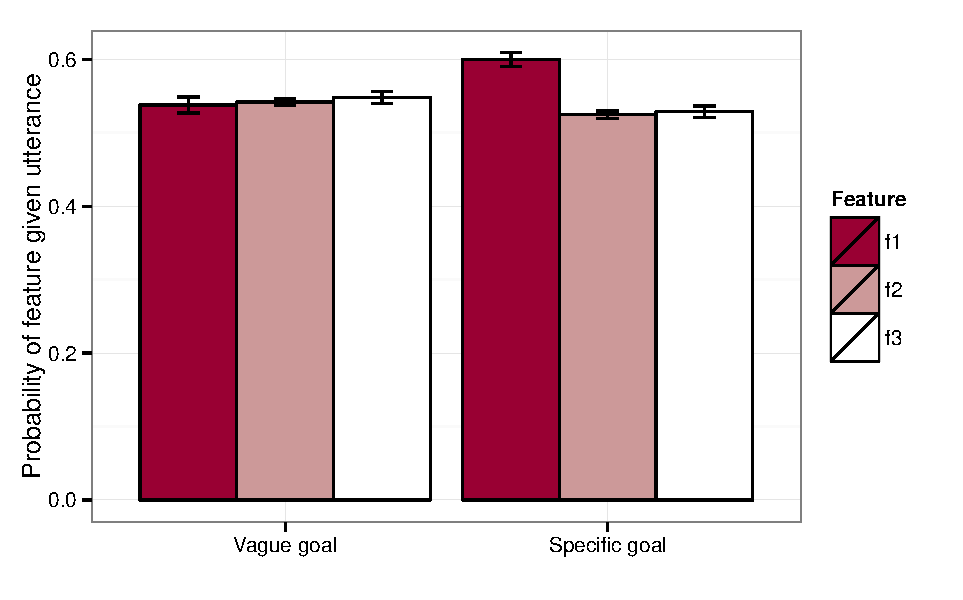
\includegraphics{Plots/model_bar.pdf}}
\end{center}
\caption{This is a figure.} 
\label{model_bar}
\end{figure}

To quantitatively evaluate the model's performance on metaphorical utterances, we correlated model predictions with human ratings for each of the features given a metaphorical utterance and a vague or specific QUD. We first focused on the model's performance on features that are $f_1$s, namely the most salient features and ones that are sometimes specifically under discussion. Correlation between human ratings and the model's marginal posterior probabilities for $f_1$ across the $32$ metaphors and vague/specific QUD conditions is $0.73$ (add Spearman prophecy formula), suggesting that the model captures a significant amount of the reliable variance in the human data. We then compare this with baseline models that only consider feature priors of the source (animal category) or target (person category). A baseline model consisting of only feature priors for the animal categories yields a non-significant correlation ($r=-0.03, p > 0.05$). A baseline model consisting of only feature priors for the person category yields a significant correlation ($r=0.59, p < 0.01$), but one that is significantly worse than the model predictions ($p < 0.001$ with a Cox test). A linear regression model that takes both sets of priors as predictors still yield a significantly worse fit than our model. This suggests that our model adequately combines prior knowledge about the source and target domains to produce metaphor interpretations that closely fit that of humans.
\begin{figure}[ht]
\begin{center}
\scalebox{0.6}{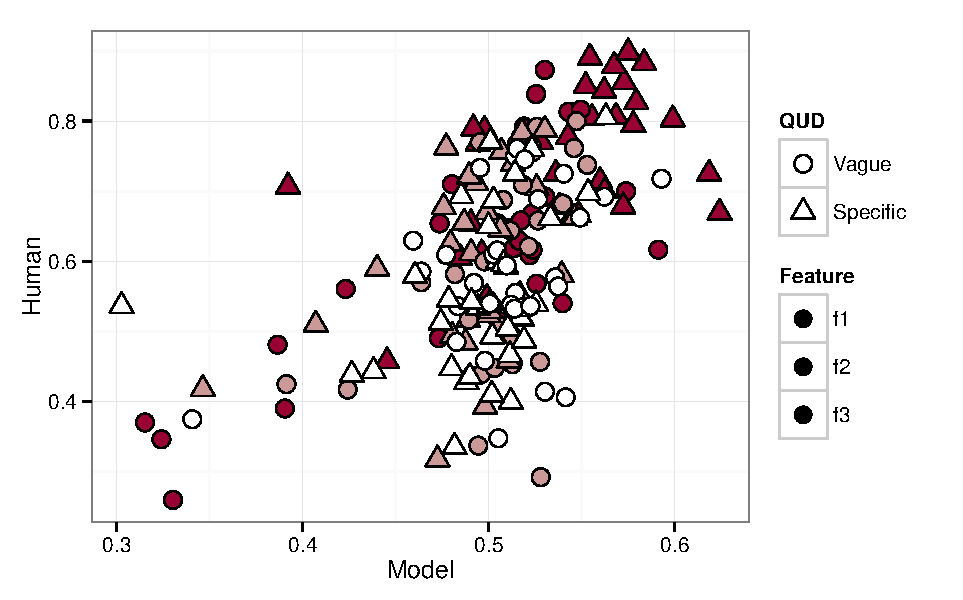
\includegraphics{Plots/scatter_full.pdf}}
\end{center}
\caption{This is a figure.} 
\label{scatter_full}
\end{figure}

We then evaluate the model's performance on all three types of features. Correlation between human ratings and the model's marginal posterior probabilities for $f_1$, $f_2$, and $f_3$ across the $32$ metaphors and vague/specific QUD conditions is $0.56$ (add Spearman prophecy formula). Figure~\ref{scatter_full} shows the model predictions against human ratings for the three features of each metaphor given a vague or specific QUD. While our model still captures a significant amount of reliable variance in the human data, we see that there are certain features, particularly $f_2$ and $f_3$, for which the model performance is significantly worse. We analyze these metaphors and features in more detail in the following section.






\section{Discussion}
Discuss implication of results on the pragmatics of metaphor; discuss other effects we could explore using the modeling framework; suggest future directions.

In this paper we focus on developing a computational model of pragmatics that explains a range of effects in metaphor understanding, with the goal of advancing our understanding of the computational basis of metaphor and nonliteral language understanding.

\subsection{Footnotes}


%\subsection{Tables}

%\begin{table}[!ht]
%\begin{center} 
%\caption{Sample table title.} 
%\label{sample-table} 
%\vskip 0.12in
%\begin{tabular}{ll} 
%\hline
%Error type    &  Example \\
%\hline
%Take smaller        &   63 - 44 = 21 \\
%Always borrow~~~~   &   96 - 42 = 34 \\
%0 - N = N           &   70 - 47 = 37 \\
%0 - N = 0           &   70 - 47 = 30 \\
%\hline
%\end{tabular} 
%\end{center} 
%\end{table}


\section{Acknowledgments}

Place acknowledgments (including funding information) in a section at
the end of the paper.


\section{References}


\bibliographystyle{apacite}

\setlength{\bibleftmargin}{.125in}
\setlength{\bibindent}{-\bibleftmargin}

\bibliography{CogSci_Template}


\end{document}
